\section{Part 2: Text document classification}
For the top twenty words with the highest likelihoods for each class, the words are not listed in any order based on likelihood.
\subsection{Part 2.1}
\subsubsection{Multinomial Naive Bayes}
\paragraph{Spam detection \\}
Overall accuracy: 0.976923076923

\begin{tabular}{l|r|r}
Class & 0 & 1 \\
\hline
Classification accuracy & 0.9538461538 & 1.0000000000 \\
\end{tabular}

Confusion matrix:

\begin{tabular}{l|r|r}
 & 0 & 1 \\
\hline
0 & 0.9538461538 & 0.0461538462 \\
1 & 0.0000000000 & 1.0000000000 \\
\end{tabular}

\begin{multicols*}{2}
Top 20 words with highest likelihood for class 0
\begin{itemize}
  \item e
  \item first
  \item follow
  \item university
  \item information
  \item fax
  \item send
  \item question
  \item call
  \item linguistic
  \item please
  \item word
  \item d
  \item www
  \item contact
  \item s
  \item provide
  \item interest
  \item http
  \item english
\end{itemize}

Top 20 words with highest likelihood for class 1
\begin{itemize}
  \item mail
  \item here
  \item need
  \item thank
  \item free
  \item our
  \item remove
  \item com
  \item receive
  \item today
  \item please
  \item information
  \item subject
  \item offer
  \item day
  \item list
  \item wish
  \item us
  \item http
  \item call
\end{itemize}
\end{multicols*}

\paragraph{Movie reviews \\}
Overall accuracy: 0.755

\begin{tabular}{l|r|r}
Class & -1 & 1 \\
\hline
Classification accuracy & 0.7420000000 & 0.7680000000 \\
\end{tabular}

Confusion matrix:

\begin{tabular}{l|r|r}
 & 0 & 1 \\
\hline
0 & 0.7420000000 & 0.2580000000 \\
1 & 0.2320000000 & 0.7680000000 \\
\end{tabular}

\begin{multicols*}{2}
Top 20 words with highest likelihood for class -1
\begin{itemize}
  \item bad
  \item never
  \item much
  \item time
  \item characters
  \item plot
  \item film
  \item story
  \item movie
  \item even
  \item nothing
  \item script
  \item comedy
  \item little
  \item one
  \item makes
  \item made
  \item would
  \item good
  \item like
\end{itemize}

Top 20 words with highest likelihood for class 1
\begin{itemize}
  \item way
  \item makes
  \item story
  \item best
  \item work
  \item film
  \item time
  \item funny
  \item one
  \item --
  \item characters
  \item even
  \item make
  \item movie
  \item performances
  \item much
  \item life
  \item good
  \item comedy
  \item like
\end{itemize}
\end{multicols*}{2}


\subsubsection{Bernoulli Naive Bayes}
\paragraph{Spam detection \\}
Overall accuracy: 0.973076923077

\begin{tabular}{l|r|r}
Class & 0 & 1 \\
\hline
Classification accuracy & 0.9538461538 & 0.9923076923 \\
\end{tabular}

Confusion matrix:

\begin{tabular}{l|r|r}
 & -1 & 1 \\
\hline
0 & 0.9538461538 & 0.0461538462 \\
1 & 0.0076923077 & 0.9923076923 \\
\end{tabular}

\begin{multicols*}{2}
Top 20 words with highest likelihood for class 0
\begin{itemize}
  \item e
  \item language
  \item university
  \item information
  \item email
  \item s
  \item fax
  \item english
  \item linguistic
  \item please
  \item address
  \item research
  \item call
  \item interest
  \item www
  \item one
  \item include
  \item http
  \item word
  \item follow
\end{itemize}

Top 20 words with highest likelihood for class 1
\begin{itemize}
  \item address
  \item s
  \item email
  \item list
  \item com
  \item http
  \item one
  \item here
  \item our
  \item send
  \item remove
  \item over
  \item please
  \item free
  \item us
  \item receive
  \item day
  \item need
  \item information
  \item mail
\end{itemize}
\end{multicols*}

\paragraph{Movie reviews \\}
Overall accuracy: 0.757

\begin{tabular}{l|r|r}
Class & -1 & 1 \\
\hline
Classification accuracy & 0.7420000000 & 0.7720000000 \\
\end{tabular}

Confusion matrix:

\begin{tabular}{l|r|r}
& -1 & 1 \\
\hline
0 & 0.7420000000 & 0.2580000000 \\
1 & 0.2280000000 & 0.7720000000 \\
\end{tabular}

\begin{multicols*}{2}
Top 20 words with highest likelihood for class -1
\begin{itemize}
  \item little
  \item never
  \item much
  \item time
  \item one
  \item plot
  \item film
  \item would
  \item nothing
  \item even
  \item bad
  \item --
  \item characters
  \item good
  \item movie
  \item comedy
  \item makes
  \item make
  \item like
  \item story
\end{itemize}

Top 20 words with highest likelihood for class 1
\begin{itemize}
  \item way
  \item comedy
  \item even
  \item best
  \item make
  \item film
  \item story
  \item funny
  \item work
  \item --
  \item time
  \item movie
  \item like
  \item one
  \item performances
  \item much
  \item life
  \item good
  \item makes
  \item characters
\end{itemize}
\end{multicols*}


\subsection{Part 2.2}
\subsubsection{Multinomial Naive Bayes}
Overall accuracy: 0.855513307985

\begin{tabular}{l|r|r|r|r}
Class & 0 & 1 & 2 & 3 \\
\hline
Classification accuracy & 0.9117647059 & 0.6363636364 & 0.9166666667 & 0.8571428571 \\
\end{tabular}

\begin{tabular}{l|r|r|r|r}
Class & 4 & 5 & 6 & 7 \\
\hline
Classification accuracy & 0.9787234043 & 0.4000000000 & 0.9130434783 & 0.8275862069 \\
\end{tabular}

Confusion matrix:

\paragraph{Left half of confusion matrix}
\begin{tabular}{l|r|r|r|r}
 & 0 & 1 & 2 & 3 \\
\hline
0 & 0.9117647059 & 0.0000000000 & 0.0000000000 & 0.0000000000 \\
1 & 0.0303030303 & 0.6363636364 & 0.0000000000 & 0.0606060606 \\
2 & 0.0000000000 & 0.0000000000 & 0.9166666667 & 0.0000000000 \\
3 & 0.0000000000 & 0.0000000000 & 0.0000000000 & 0.8571428571 \\
4 & 0.0212765957 & 0.0000000000 & 0.0000000000 & 0.0000000000 \\
5 & 0.2000000000 & 0.1000000000 & 0.0000000000 & 0.1000000000 \\
6 & 0.0000000000 & 0.0000000000 & 0.0000000000 & 0.0000000000 \\
7 & 0.0344827586 & 0.0000000000 & 0.0000000000 & 0.0000000000 \\
\end{tabular}

\paragraph{Right half of confusion matrix}
\begin{tabular}{l|r|r|r|r}
 & 4 & 5 & 6 & 7 \\
\hline
0 & 0.0882352941 & 0.0000000000 & 0.0000000000 & 0.0000000000 \\
1 & 0.1818181818 & 0.0000000000 & 0.0000000000 & 0.0909090909 \\
2 & 0.0555555556 & 0.0000000000 & 0.0000000000 & 0.0277777778 \\
3 & 0.0357142857 & 0.0000000000 & 0.0000000000 & 0.1071428571 \\
4 & 0.9787234043 & 0.0000000000 & 0.0000000000 & 0.0000000000 \\
5 & 0.1000000000 & 0.4000000000 & 0.0000000000 & 0.1000000000 \\
6 & 0.0652173913 & 0.0000000000 & 0.9130434783 & 0.0217391304 \\
7 & 0.1379310345 & 0.0000000000 & 0.0000000000 & 0.8275862069 \\
\end{tabular}

\begin{multicols*}{2}
Top 20 words with highest likelihood for class 0
\begin{itemize}
  \item much
  \item article
  \item something
  \item one
  \item make
  \item get
  \item like
  \item would
  \item think
  \item subject
  \item could
  \item well
  \item ca
  \item also
  \item m
  \item way
  \item know
  \item writes
  \item new
  \item see
\end{itemize}

Top 20 words with highest likelihood for class 1
\begin{itemize}
  \item could
  \item think
  \item use
  \item article
  \item even
  \item two
  \item anyone
  \item would
  \item nt
  \item know
  \item one
  \item get
  \item good
  \item writes
  \item like
  \item also
  \item subject
  \item work
  \item well
  \item want
\end{itemize}

Top 20 words with highest likelihood for class 2
\begin{itemize}
  \item one
  \item see
  \item know
  \item last
  \item even
  \item really
  \item baseball
  \item many
  \item would
  \item think
  \item article
  \item m
  \item say
  \item edu
  \item time
  \item like
  \item get
  \item writes
  \item subject
  \item first
\end{itemize}

Top 20 words with highest likelihood for class 3
\begin{itemize}
  \item subject
  \item like
  \item need
  \item using
  \item fax
  \item would
  \item article
  \item help
  \item know
  \item m
  \item following
  \item use
  \item one
  \item x
  \item writes
  \item also
  \item problem
  \item nt
  \item get
  \item thanks
\end{itemize}

Top 20 words with highest likelihood for class 4
\begin{itemize}
  \item many
  \item people
  \item one
  \item even
  \item ca
  \item writes
  \item m
  \item also
  \item much
  \item time
  \item like
  \item could
  \item get
  \item go
  \item article
  \item subject
  \item way
  \item think
  \item well
  \item know
\end{itemize}

Top 20 words with highest likelihood for class 5
\begin{itemize}
  \item edu
  \item following
  \item shipping
  \item like
  \item price
  \item used
  \item please
  \item nt
  \item email
  \item good
  \item get
  \item new
  \item subject
  \item condition
  \item sale
  \item want
  \item send
  \item interested
  \item university
  \item know
\end{itemize}

Top 20 words with highest likelihood for class 6
\begin{itemize}
  \item see
  \item writes
  \item first
  \item like
  \item article
  \item even
  \item hockey
  \item last
  \item one
  \item play
  \item well
  \item contact
  \item nhl
  \item way
  \item time
  \item games
  \item going
  \item subject
  \item team
  \item would
\end{itemize}

Top 20 words with highest likelihood for class 7
\begin{itemize}
  \item like
  \item would
  \item one
  \item two
  \item also
  \item think
  \item make
  \item get
  \item writes
  \item anyone
  \item well
  \item could
  \item m
  \item know
  \item email
  \item much
  \item subject
  \item thanks
  \item nt
  \item article
\end{itemize}
\end{multicols*}

\subsubsection{Bernoulli Naive Bayes}
Overall accuracy: 0.863117870722

\begin{tabular}{l|r|r|r|r}
Class & 0 & 1 & 2 & 3 \\
\hline
Classification accuracy & 0.9117647059 & 0.6060606061 & 0.8888888889 & 0.7142857143 \\
\end{tabular}

\begin{tabular}{l|r|r|r|r}
Class & 4 & 5 & 6 & 7 \\
\hline
Classification accuracy & 0.9574468085 & 0.7000000000 & 0.9347826087 & 1.0000000000 \\
\end{tabular}

Confusion matrix:

\paragraph{Left side of confusion matrix}
\begin{tabular}{l|r|r|r|r}
 & 0 & 1 & 2 & 3 \\
\hline
0 & 0.9117647059 & 0.0000000000 & 0.0000000000 & 0.0000000000 \\
1 & 0.0000000000 & 0.6060606061 & 0.0000000000 & 0.0000000000 \\
2 & 0.0000000000 & 0.0000000000 & 0.8888888889 & 0.0000000000 \\
3 & 0.0000000000 & 0.0000000000 & 0.0000000000 & 0.7142857143 \\
4 & 0.0212765957 & 0.0000000000 & 0.0000000000 & 0.0000000000 \\
5 & 0.0000000000 & 0.1000000000 & 0.0000000000 & 0.0000000000 \\
6 & 0.0000000000 & 0.0000000000 & 0.0000000000 & 0.0000000000 \\
7 & 0.0000000000 & 0.0000000000 & 0.0000000000 & 0.0000000000 \\
\end{tabular}

\paragraph{Right side of confusion matrix}
\begin{tabular}{l|r|r|r|r}
 & 4 & 5 & 6 & 7\\
\hline
0 & 0.0294117647 & 0.0000000000 & 0.0000000000 & 0.0588235294 \\
1 & 0.0000000000 & 0.0000000000 & 0.0000000000 & 0.3939393939 \\
2 & 0.0277777778 & 0.0000000000 & 0.0000000000 & 0.0833333333 \\
3 & 0.0000000000 & 0.0000000000 & 0.0000000000 & 0.2857142857 \\
4 & 0.9574468085 & 0.0000000000 & 0.0000000000 & 0.0212765957 \\
5 & 0.0000000000 & 0.7000000000 & 0.0000000000 & 0.2000000000 \\
6 & 0.0434782609 & 0.0000000000 & 0.9347826087 & 0.0217391304 \\
7 & 0.0000000000 & 0.0000000000 & 0.0000000000 & 1.0000000000 \\
\end{tabular}

\begin{multicols*}{2}
Top 20 words with highest likelihood for class 0
\begin{itemize}
  \item much
  \item edu
  \item get
  \item subject
  \item m
  \item also
  \item new
  \item one
  \item way
  \item nt
  \item article
  \item space
  \item see
  \item like
  \item could
  \item time
  \item think
  \item would
  \item us
  \item writes
\end{itemize}

Top 20 words with highest likelihood for class 1
\begin{itemize}
  \item know
  \item subject
  \item system
  \item article
  \item edu
  \item think
  \item like
  \item nt
  \item card
  \item work
  \item problem
  \item get
  \item use
  \item one
  \item drive
  \item writes
  \item would
  \item also
  \item m
  \item two
\end{itemize}

Top 20 words with highest likelihood for class 2
\begin{itemize}
  \item good
  \item time
  \item get
  \item m
  \item writes
  \item game
  \item first
  \item edu
  \item year
  \item article
  \item last
  \item subject
  \item baseball
  \item team
  \item one
  \item know
  \item would
  \item think
  \item nt
  \item like
\end{itemize}

Top 20 words with highest likelihood for class 3
\begin{itemize}
  \item use
  \item one
  \item using
  \item also
  \item know
  \item writes
  \item m
  \item set
  \item subject
  \item get
  \item nt
  \item code
  \item like
  \item window
  \item article
  \item help
  \item email
  \item x
  \item would
  \item problem
\end{itemize}

Top 20 words with highest likelihood for class 4
\begin{itemize}
  \item one
  \item know
  \item time
  \item writes
  \item m
  \item think
  \item could
  \item get
  \item even
  \item us
  \item nt
  \item make
  \item would
  \item article
  \item much
  \item people
  \item like
  \item edu
  \item government
  \item subject
\end{itemize}

Top 20 words with highest likelihood for class 5
\begin{itemize}
  \item condition
  \item used
  \item get
  \item new
  \item list
  \item use
  \item shipping
  \item email
  \item like
  \item price
  \item nt
  \item good
  \item edu
  \item one
  \item etc
  \item want
  \item subject
  \item please
  \item know
  \item sale
\end{itemize}

Top 20 words with highest likelihood for class 6
\begin{itemize}
  \item like
  \item first
  \item nhl
  \item hockey
  \item time
  \item nt
  \item article
  \item game
  \item team
  \item last
  \item go
  \item writes
  \item one
  \item think
  \item get
  \item subject
  \item would
  \item games
  \item play
  \item year
\end{itemize}

Top 20 words with highest likelihood for class 7
\begin{itemize}
  \item need
  \item computer
  \item program
  \item two
  \item like
  \item would
  \item article
  \item nt
  \item also
  \item use
  \item one
  \item edu
  \item writes
  \item m
  \item know
  \item subject
  \item could
  \item graphics
  \item think
  \item get
\end{itemize}
\end{multicols*}

\subsection{Extra credit}
Using the WordCloud Python package, we created word clouds from the test documents.
\subsubsection{Word cloud of spam detection's test set documents.}
\begin{figure}[H]
  \centering
  
\includegraphics[width=1\textwidth]{graphics/spam_matplotlib.png}
  \caption{With matplotlib.}
\end{figure}
\begin{figure}[H]
  \centering
  
\includegraphics[width=1\textwidth]{graphics/spam_reduced.png}
  \caption{With reduced font size.}
\end{figure}

\subsubsection{Word cloud of movie reviews' test set documents.}
\begin{figure}[H]
  \centering
  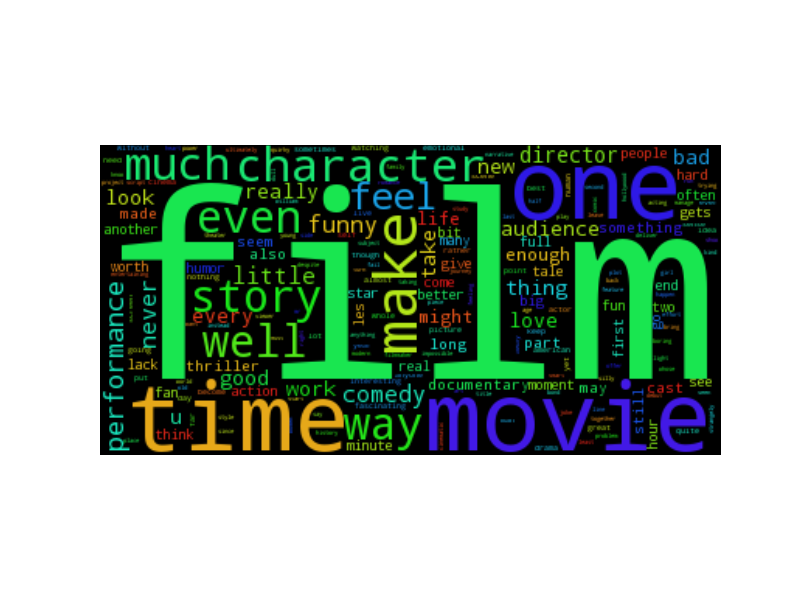
\includegraphics[width=1\textwidth]{graphics/sentiment_matplotlib.png}
  \caption{With matplotlib.}
\end{figure}
\begin{figure}[H]
  \centering
  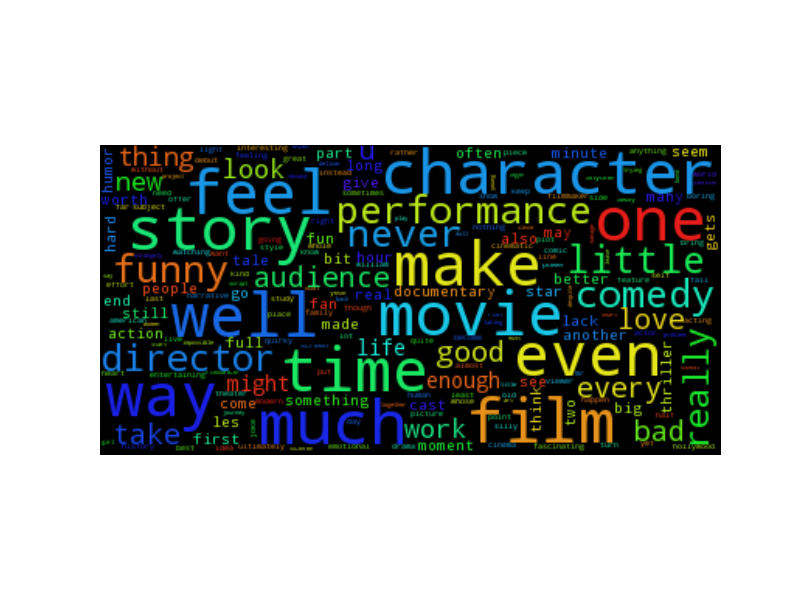
\includegraphics[width=1\textwidth]{graphics/sentiment_reduced.png}
  \caption{With reduced font size.}
\end{figure}